\documentclass[a4paper]{article}

\usepackage[utf8]{inputenc}

\usepackage{url}
\usepackage[hidelinks]{hyperref}

\usepackage{caption}

\usepackage{listings}

\usepackage{color}

% *** GRAPHICS RELATED PACKAGES ***
%\usepackage[pdftex]{graphicx}
\usepackage{graphicx}
%\usepackage[dvips]{graphicx}
% to place figures on a fixed position
\usepackage{float}

\usepackage[margin=1in]{geometry}

\title{Testing of Network Services}
\author{}
\date{}


\begin{document}

\lstdefinelanguage{TTCN3}
{
  morekeywords={
    import,from,all,
    integer,boolean,bitstring,charstring,false,true,omit,
    var,const,type,record,set,union,enumerated,of,
    template,modifies,
    port,message,in,out,inout,component,timer,map,create,connect,unmap,
    function,return,runs,on,testcase,system,control,execute,self,
    send,receive,timeout,pass,fail,inconc,alt,value,start,stop,
    and,or,if,else,
    fail,pass,inconc,setverdict,log,
    int2float,int2str,int2char,lengthof,str2int
  },
  sensitive=true, % keywords are not case-sensitive
  morecomment=[l]{//}, % l is for line comment
  morecomment=[s]{/*}{*/}, % s is for start and end delimiter
  morestring=[b]" % defines that strings are enclosed in double quotes
}
\lstset{language=TTCN3}
\lstset{frame=single}
\lstset{breaklines=true}
\lstset{backgroundcolor=\color{yellow}}
\lstset{keywordstyle=\color{blue}\bf}

\maketitle

\tableofcontents

\section{Introduction}

The purpose of this lab is to give an insight on system test and to be a teaser to the world of script based automated
test execution. During this lab we are going to test LAP-B protocol which is the second layer of the X.25 protocol
stack. What makes this lab exotic is that the transmission medium of the protocol is not going to be a physical layer
but HTTP instead. The protocol entity to be tested is a web application running on a server : JSON text inside HTTP
POST messages can be used for sending LAP-B frames destined for the device under test that will respond with frames in
JSON data in HTTP likewise. As consequence this architecture will give insight on:
\begin{itemize}
    \item script based black-box testing
    \item automated testing of web applications
    \item the application of a generic purpose test execution environment - Ericsson TITAN
    \item TTCN-3 test description language
\end{itemize}

\section{Lab environment}

The software and hardware components that are used during this lab can be seen on Fig.~\ref{fig:lab-arch}.
A virtual machine -- with Ubuntu Linux installed -- is used that contains an Ericsson TITAN test execution environment,
a TITAN Eclipse plug-in that is used for creating test scripts and for controlling the execution. As TITAN is a general
purpose test execution framework a \emph{test port} has to be used for defining the way of message transmission and
reception that are used in the test cases. Since a web server is on the receiving end of the communication the TITAN
HTTP port is used for that purpose.

The system under test is LAP-B protocol over HTTP reachable on \url{152.66.246.231:3000}. It is advised to take a look
on this page before the measurements and experiment with the protocol operation over the web UI -- without using the
JSON API.
Each state of the LAP-B protocol corresponds to a web page and the state transitions can be triggered by sending data
through the HTML forms.
This web application uses cookies for storing the state so previously started sessions can be continued until deleting
the cookies.

The web application has an additional JSON web service API that is used for verifying the correctness of the protocol's
behavior.

The login credentials for the VM (user/pass): \textbf{\emph{ttcn/ttcn}}

\begin{figure}[!htb]
    \centering
    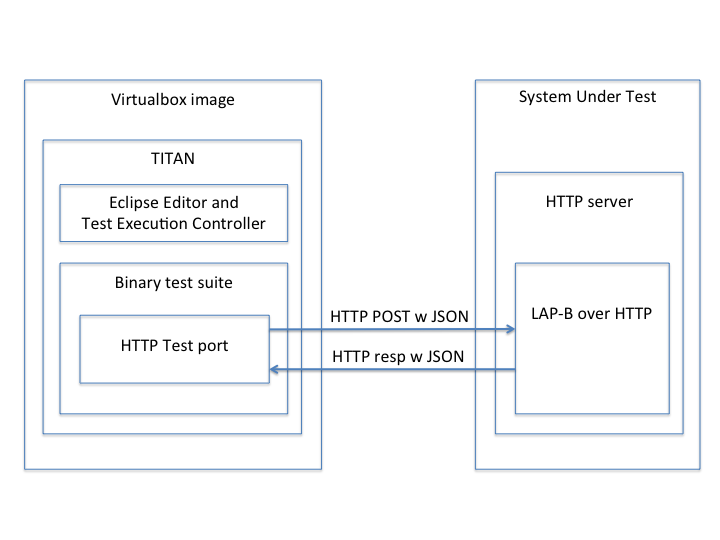
\includegraphics[width=0.9\textwidth]{figures/lab-arch.png}
    \caption{The architecture of the lab}
    \label{fig:lab-arch}
\end{figure}

\section{Testing, protocol testing, web service testing}

\subsection{System test}

The purpose of system test is to make a verdict on the test candidate system in terms of conformance with the
functional and non-functional specification. During system test the test candidate is only accessed through its
external interfaces -- the internal state is unknown at any time point, it acts like a black box.

When testing the test environment (\emph{tester} in the following) sees the System Under Test (\emph{SUT}) as a
black-box. The tester can only send and receive messages from the direction of the SUT through the Point of Control and
Observations (PCO). The conformance is verified only through the observable behavior of the SUT over the PCOs.
In a system test the operations declared in the public interface of the system can be executed in an arbitrary sequence
with arbitrarily many times therefore the possible sequence and length of an event vector is unbounded/infinite. The
result of such unbounded event vector can not be verified therefore a representative selection of them is made what is
called \emph{test suite}. The hypothesis is that a thorough test suite guarantees the system's conformance with the
specs with high probability.

\subsection{Black-box testing}

In order to execute a test a test suite has to be created. The structure of a test suite is a hierarchy whose basic
component is called \emph{test case}. Each test case has a \emph{test purpose} that is basically checking that SUT
satisfies one of the criteria of the system specification. Test cases can be further break down into \emph{test steps}
that can contain further test steps recursively or \emph{test events}. Test events are considered to be at the lowest
level of the hierarchy and to be atomic.
For example a test event can be a reception of a protocol message or sending one, the expiry of a timer etc. The
sequence of these atomic test events can be combined into a test step arbitrarily.

The operations executed during a test case run can be split into four phases:
\begin{itemize}
    \item Reset the system. Some protocols have reset message others don't. In that case an appropriate message
          sequence
          has to be executed that guarantees to drive the protocol's state machine into the starting state.
    \item Prefix event sequence: the system is driven from the starting state to the state where the goal of the test
          purpose is verified. This is usually the shortest event sequence denoted by the spanning tree of the system's
          state
          machine originated from the starting state.
    \item Execute the operations that verifies the completion of the test case's goal and check whether the system
          responded appropriately.
    \item We are not done yet at this point! We have to check as a post-condition that the system ended up in the
          correct
          state that is checked using a post-condition operations sequence.
\end{itemize}

Telecommunication systems are non-deterministic due to non-error free data transmission and the occurrence of
non-deterministic delays over the communication channels. Errors can occur such as data corruption or message loss
caused by a bit error in the physical layer or message duplication or reordering of messages because of other reasons.
As a consequence beside of the positive outcome a test case must be prepared for handling unexpected events as a result
of message sending. All messages sent have to be protected with a timer so that in case of a message loss or deadlock
in the SUT it won't not block the tester and the test execution.

The output of the test case execution is the \emph{verdict}. The hypothesis is that if a system responded with the
correct output during the 4 phases described above then our terminal state was correct resulting in a \emph{pass}
verdict of the test case. If we receive an unexpected message during any message exchange the test case ends in a
\emph{fail} verdict also blocking further execution of steps. If the system failed to respond to a request -- that
could be caused by network congestion -- it can not be decided whether the operation was correct or not. In such case
the verdict is \emph{inconclusive}. There are two more verdicts: \emph{none} when there is no verdict as a result of a
test case and \emph{error} where some error occurred during test case execution.

\subsection{Testing of web portals}

The testing of web portals are mostly checking user stories that appear as a browsing process for the the testers. Even
today the testing process is mostly manual but there are several frameworks exist for script based automation. The
browsing process is split into test steps that are basically raising events sequentially that are visible on the page.
The source of an event can be something like following a link, filling out and submitting a form or some other
JavaScript based event. During the browsing process the test verifies that as a result of following a link the correct
page is shown that has the expected content.

The testing of web portals and protocols are analogous. The web portal can be viewed as a black box from the user's
perspective where the user can't peek into the back-end database. The web portal can also be viewed as a state machine
where a state is a concrete view of the portal that is a result of the similar URIs visible in the browser's search
bar. The navigation between the pages can be seen as the state transitions of the state machines. A state transition is
made out of 2 messages: a HTTP request and a corresponding HTTP response. The message types are classified based on the
URI found in the request and the message formats are defined by the format of the HTTP request body format. The
precondition phase of a test case is navigating to the given site  and the postcondition phase verifies that the page
view after the given user event under test is correct or not.
When testing web portal there are only 3 possible verdicts:
\begin{itemize}
    \item \emph{pass}, if the navigation to the destination site was OK, and the resulting content was the expected
    \item \emph{fail}, when either the navigation fails or the content mismatches
    \item \emph{error}, when the web portal returns with an unexpected error code or present an error page
\end{itemize}

The main difference between testing web portals and telecommunication protocols is that while the former one is always
deterministic the latter one is non-deterministic due to the nature of the underlying non-reliable medium. Another
difference is that while testing protocols enough time must be provided for the response messages to arrive due to
network latency and deadlock evasion so timers are utilized extensively. When testing web portals these effects has
lesser significance as a consequence timers are used less frequently.

\section{LAP-B}

During this lab the implementation of  \emph{Link Access Procedure, Balanced} (LAPB) is going to be tested. LAPB is the
X.25 protocol stack's data link layer protocol with HDLC framing. This protocol is rarely used nowadays but it still
can be used for demonstrating protocol entity operation. LAPB provides connection oriented, bit based, reliable,
in-order transmission service with error detection between a \emph{Data Terminal Equipment} (DTE) and a \emph{Data
    Circuit-terminating Equipment}. For higher level protocols it provides the following service primitives:
\begin{itemize}
    \item connect request
    \item disconnect request
    \item data request (request data transmission)
\end{itemize}
Towards upper layer protocols it provides the following indications:
\begin{itemize}
    \item connect indication
    \item disconnect indication
    \item connect confirmation
    \item disconnect confirmation
    \item data indication
\end{itemize}

\subsection{Message types and frame formats}

The frame data is encapsulated in 01111110 (0x7E) flag. For transparent data transmission inside the frame body the
sending device inserts a 0 bit after each consecutive 1 bit that are removed at the receiving side (this is called bit
stuffing).

LAP-B frames have 4 main parts as seen on Figure~\ref{fig:lapbframe}. The first part is the address field followed by
the control field followed by the information field -- that is present only in some of the frame types. The frame's
last component is a 2 byte frame check sequence.

\begin{figure}[!htb]
    \centering
    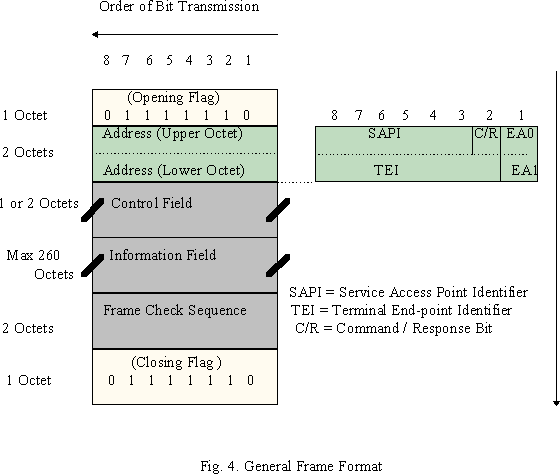
\includegraphics[width=0.9\textwidth]{figures/lapbframe.png}
    \caption{The structure of LAP-B frames}
    \label{fig:lapbframe}
\end{figure}

The address field determines the direction of the communication (DTE-DCE or DCE-DTE) and whether the message is
multicast or not. Furthermore it has a C/R bit that indicates whether the frame is a command or a request.

The control field carries an ID that discriminates the type of the frame and a sequence number that is required for
detecting and correcting missing frames. LAP-B utilizes three different types of frames:
\begin{itemize}
    \item U frame (Unnumbered). This frame type is used for establishing and disconnecting	LAP-B connections and
          also for
          sending acknowledgments.
    \item I frame (Information). This frame type is used for transparent transmission of the network layer protocol
          data
          units.
    \item S frame (Supervisory). This frame type is used for controlling the transmission of I frames in terms of
          congestion and flow control.
\end{itemize}

The control field has 3 different format corresponding to the frame types above. The common part in each that they have
a P/F (Poll/Final) bit. A sender of a frame with P=1 expects the peer to respond with a frame that has F=1. When P=0
the sender does not expect the peer to respond. For unsolicited response messages (e.g. error indication) F=0.
The unnumbered frame's control field contains a message type field that can have the following values:
\begin{itemize}
    \item SABM: command frame to establish connection between the DTE and DCE using modulo 8 sequence numbering
    \item SABME: command frame to establish connection between the DTE and DCE using modulo 128 sequence numbering
    \item UA: response frame for acknowledging the connection establishment or disconnection
    \item DISC: command frame for disconnecting a connection
    \item DM: response frame for acknowledging the connection establishment or disconnection
          (kind of similar to UA, for some messages UA is a positive acknowledgment and DM is the negative and for some
          others
          vice versa)
    \item FRMR: response frame for error indication
\end{itemize}

The I frame's control field carries two sequence numbers: the seq. no. of the sent frame -- N(S) -- and the seq. no. of
the next expected frame -- N(R).
N(R) simultaneously serves as an acknowledgment of receiving frames up until N(R)-1.

The supervisory frame's control field contains a message type and an expected seq. no. field that can be used for
positive acknowledgment similarly to I frames. Based on the message type field the following supervisory frames are
recognized:
\begin{itemize}
    \item RR: I frame acknowledgment if there is no message to send in the opposite direction or for signaling the end
          of
          the previously signaled RNR state's end
    \item RNR: temporarily the entity is not ready for reception of I frames
    \item REJ: request for retransmission of I frames starting from N(R)
\end{itemize}

The protocol defines two timers:
\begin{itemize}
    \item T1: the retransmission timer
    \item T2: the (\verb!pending!) status timer
\end{itemize}

\subsection{Protocol state-machine}

The protocol has two queues:
\begin{itemize}
    \item message queue: this is the queue of the not yet sent messages arriving from the upper layers
    \item acknowledgment queue: the queue of the messages sent but not yet acknowledged by the peer entity
\end{itemize}

The message get into the former queue as a result of using a data request service primitive from where the message is
transferred to the latter queue as result of sending an I frame. The message is removed from the queue finally when a
positive acknowledgment is received for it. Disconnection causes flushing of both queues.

The protocol has several state variables:
\begin{itemize}
    \item \verb!mode!: \verb!basic! - means that 3 bit sequence numbers or
          \verb!extended! is in use (7 bit seq. no.)
    \item (\verb!busy!) status: there was a congestion during data processing
    \item (\verb!rejecting!) status: subsequent data transmission is not possible to a previous error
    \item (\verb!pending!) status: there are processed but not yet acknowledged messages, acknowledgment
          has to
          be sent
    \item (\verb!window!): integer variable, determines the maximal size of the sent but not acknowledged
          buffer
    \item \verb!vs!: the sequence no. of the last sent message, last element in the acknowledgment
          queue
    \item \verb!va!: sequence number of the oldest unacknowledged message, the first element in the
          acknowledgment queue
    \item \verb!vr!: the expected seq. no. in the last received message
    \item \verb!n2!: the maximal retransmission count of a message
    \item \verb!n2_count!: the retry count of the last sent message
\end{itemize}

The protocol has 5 states that define the state of the data connection:
\begin{itemize}
    \item disconnected: both sides are in disconnected state, starting state
    \item disconnecting: the disconnection is half-way done, the entity is waiting for the peer to acknowledge the
          disconnect request
    \item connecting): the connection is half-open, one side is waiting for the other for a positive acknowledgment for
          the
          connection initiation request
    \item connected: both sides are in connected state, data transmission is possible
    \item frame reject: temporary error on either side, rejects all request until re-connection
\end{itemize}

The processing of service primitives from the upper layers are permitted in every state. The state transition table is
detailed further down. The columns stand for the the messages the rows represent the current state. The cell value
holds the index of the next state and the sent message separated by \verb./. symbol. The data
request primitive sends the next message in the message queue not the one that's currently under reception.

{\footnotesize
\begin{center}
    \begin{tabular}{|l|c|c|c|}
        \hline
                          & \verb!connect_request! & \verb!disconnect_request! & \verb!data_request!  \\
        \hline
        disconnected (0)  & 1/SABM or SABME             & 0/-                         & 0/-                          \\
        \hline
        connecting (1)    & 1/-                         & 0/DISC                      & 2/-                          \\
        \hline
        disconnecting (2) & 1/SABM or SABME             & 0/-                         & 2/-                          \\
        \hline
        connected (3)     & 3/-                         & 2/DISC                      & 3/I                          \\
        \hline
        frame reject (4)  & 4/-                         & 2/DISC                      & 4/I                          \\
        \hline
    \end{tabular}
\end{center}
}

The SABM message has to replied with a UA message towards the peer and a \verb!connect_indication! has to be signaled
towards the upper layer client if the \verb!mode! state variable is \verb/basic/. The
response is DM if the \verb!mode! is \verb/extended/.

{\footnotesize
\begin{center}
    \begin{tabular}{|l|c|c|}
        \hline
        SABM              & mode=basic                           & mode=extended  \\
        \hline
        disconnected (0)  & 3/UA and \verb!connect_indication! & 0/DM           \\
        \hline
        connecting (1)    & 1/UA and I                           & 1/DM and I     \\
        \hline
        disconnecting (2) & 2/DM                                 & 2/DM           \\
        \hline
        connected (3)     & 3/UA and I                           & 3/DM and I     \\
        \hline
        frame reject (4)  & 3/UA                                 & 4/DM           \\
        \hline
    \end{tabular}
\end{center}
}

In case of a SABME message everything is the other way around.

{\footnotesize
\begin{center}
    \begin{tabular}{|l|c|c|}
        \hline
        SABME             & mode=basic & mode=extended                         \\
        \hline
        disconnected (0)  & 0/DM       & 3/UA and \verb!connect_indication!  \\
        \hline
        connecting (1)    & 1/UA and I & 1/DM and I                            \\
        \hline
        disconnecting (2) & 2/DM       & 2/DM                                  \\
        \hline
        connected (3)     & 3/DM and I & 3/UA and I                            \\
        \hline
        frame reject (4)  & 4/DM       & 3/UA                                  \\
        \hline
    \end{tabular}
\end{center}
}

The events after receiving a DISC message is shown by the table below. During frame reject state reception of a DISC
message is not permitted. In connected state an I frame is sent if there some data to be transmitted or retransmission
is required.

{\footnotesize
\begin{center}
    \begin{tabular}{|l|c|}
        \hline
        DISC              & state/action                                \\
        \hline
        disconnected (0)  & 0/DM                                        \\
        \hline
        connecting (1)    & 1/DM and I                                  \\
        \hline
        disconnecting (2) & 2/UA                                        \\
        \hline
        connected (3)     & 0/DM and \verb!disconnect_indication! and I  \\
        \hline
        frame reject (4)  & 4/-                                         \\
        \hline
    \end{tabular}
\end{center}
}

The state transition after receiving a DM message is show in the table below. It is not permitted to receive a DISC
message in disconnected or frame reject states.In connected state an I frame is sent if there some data to be
transmitted or retransmission is required.

{\footnotesize
\begin{center}
    \begin{tabular}{|l|c|c|}
        \hline
        DM                & poll=on                             & poll=off                             \\
        \hline
        disconnected (0)  & 0/-                                 & 0/-                                  \\
        \hline
        connecting (1)    & 0/\verb!disconnect_indication! and I & 1/I                                  \\
        \hline
        disconnecting (2) & 0/\verb!disconnect_confirmation!       & 2/-                                  \\
        \hline
        connected (3)     & 0/\verb!disconnect_indication! and I & 0/\verb!disconnect_indication! and I  \\
        \hline
        frame reject (4)  & 4/-                                 & 4/-                                  \\
        \hline
    \end{tabular}
\end{center}
}

The valid state transitions upon receiving a UA message are shown in the table below. Reception of a UA frame is not
permitted in connected and frame reject states.

{\footnotesize
\begin{center}
    \begin{tabular}{|l|c|c|}
        \hline
        UA                & poll=on                             & poll=off  \\
        \hline
        disconnected (0)  & 0/-                                 & 0/-       \\
        \hline
        connecting (1)    & 3/\verb!connect_confirmation! and I & 1/I       \\
        \hline
        disconnecting (2) & 0/\verb!disconnect_confirmation!       & 2/-       \\
        \hline
        connected (3)     & 3/-                                 & 3/-       \\
        \hline
        frame reject (4)  & 4/-                                 & 4/-       \\
        \hline
    \end{tabular}
\end{center}
}

The state transitions after receiving an FRMR message are shown in the table below. Only allowed in connected state.

{\footnotesize
\begin{center}
    \begin{tabular}{|l|c|}
        \hline
        UA                & state/action  \\
        \hline
        disconnected (0)  & 0/-           \\
        \hline
        connecting (1)    & 1/-           \\
        \hline
        disconnecting (2) & 2/-           \\
        \hline
        connected (3)     & 1/I           \\
        \hline
        frame reject (4)  & 4/-           \\
        \hline
    \end{tabular}
\end{center}
}

State transitions after receiving an RR message are shown in the table below. Only allowed in states connected and
disconnecting. This table assumes $va \leq N(R) \leq vs$ otherwise the message is invalid. Reception of RR clears the
busy state, sending of an RR message clears pending status. In connected state an I frame is sent if there is any data
to be send or retransmission is required.

{\footnotesize
\begin{center}
    \begin{tabular}{|l|c|c|c|}
        \hline
        RR                & command, poll=on & response, poll=on & otherwise  \\
        \hline
        disconnected (0)  & 0/-              & 0/-               & 0/-        \\
        \hline
        connecting (1)    & 1/-              & 1/-               & 1/-        \\
        \hline
        disconnecting (2) & 2/DM             & 2/DM              & 2/-        \\
        \hline
        connected (3)     & 3/RR+I           & 3/I               & 3/I        \\
        \hline
        frame reject (4)  & 4/-              & 4/-               & 4/-        \\
        \hline
    \end{tabular}
\end{center}
}

State transitions after receiving an RNR message are shown in the table below. Only allowed in states connected and
disconnecting. This table assumes $va \leq N(R) \leq vs$ otherwise the message is invalid. Reception of RNR sets the
busy state, sending of an RR message clears pending status. In connected state an I frame is sent if there is any data
to be send or retransmission is required.

{\footnotesize
\begin{center}
    \begin{tabular}{|l|c|c|c|}
        \hline
        RNR               & command, poll=on & response, poll=on & otherwise  \\
        \hline
        disconnected (0)  & 0/-              & 0/-               & 0/-        \\
        \hline
        connecting (1)    & 1/-              & 1/-               & 1/-        \\
        \hline
        disconnecting (2) & 2/DM             & 2/DM              & 2/-        \\
        \hline
        connected (3)     & 3/RR+I           & 3/I               & 3/I        \\
        \hline
        frame reject (4)  & 4/-              & 4/-               & 4/-        \\
        \hline
    \end{tabular}
\end{center}
}

State transitions after receiving an REJ message are shown in the table below. Only allowed in states connected and
disconnecting. This table assumes $va \leq N(R) \leq vs$, otherwise the message is invalid. Reception of REJ clears the
busy state, sending of an RR message clears pending status. In connected state an I frame is sent if there is any data
to be send or retransmission is required.

{\footnotesize
\begin{center}
    \begin{tabular}{|l|c|c|c|}
        \hline
        REJ               & command, poll=on & response, poll=on & otherwise  \\
        \hline
        disconnected (0)  & 0/-              & 0/-               & 0/-        \\
        \hline
        connecting (1)    & 1/-              & 1/-               & 1/-        \\
        \hline
        disconnecting (2) & 2/DM             & 2/DM              & 2/-        \\
        \hline
        connected (3)     & 3/RR+I           & 3/I               & 3/I        \\
        \hline
        frame reject (4)  & 4/-              & 4/-               & 4/-        \\
        \hline
    \end{tabular}
\end{center}
}

Reception of an I frame is only valid in connected and disconnecting states. In disconnecting sate if the P=1 then the
response must be DM else nothing. The next state is unchanged. In connected state there are other rules to follow:

\begin{itemize}
    \item If $va \leq N(R) \leq vs$, then the message is valid, otherwise invalid
    \item If $N(S) = vr$, then we received a message with the expected seq.no. increment $vr$ by one.
          \begin{itemize}
              \item  If poll bit is set beside these RR frame is sent otherwise pending status is set.
          \end{itemize}
    \item If frame is receive with out of order sequence no.,
          \begin{itemize}
              \item if reject status is set and P=1 in the received frame an RR is sent, pending status is set and T2
                    timer is
                    started
              \item if reject status is not set then set reject status and send REJ message
          \end{itemize}
    \item If the message queue is not empty also send an I frame
\end{itemize}
In case of valid messages the next state stays the connected state.

The reception of a message with invalid FCS or	$va \geq N(R) \geq vs$ sequence number -- i.e. corrupted frame -- has
the following state transitions:

{\footnotesize
\begin{center}
    \begin{tabular}{|l|c|c|}
        \hline
        UA                & state/action  \\
        \hline
        disconnected (0)  & 0/-           \\
        \hline
        connecting (1)    & 1/-           \\
        \hline
        disconnecting (2) & 2/-           \\
        \hline
        connected (3)     & 4/I           \\
        \hline
        frame reject (4)  & 4/-           \\
        \hline
    \end{tabular}
\end{center}
}

T1 timer is responsible for message retransmission. If the current retransmission count (\verb!n2_count!)
is less than the maximal retransmission count (\verb!n2!) then the retransmission count is increased
by one and the last sent message is retransmitted.

{\footnotesize
\begin{center}
    \begin{tabular}{|l|c|c|}
        \hline
        T1                & $n2 < n2_count$ & $n2 = n2_count$                \\
        \hline
        disconnected (0)  & 0/DM            & 0/DM                           \\
        \hline
        connecting (1)    & 1/SABM or SABME & 0/\verb!disconnect_indication!  \\
        \hline
        disconnecting (2) & 2/DISC          & 0/\verb!disconnect_indication!  \\
        \hline
        connected (3)     & 3/I             & 0/\verb!disconnect_indication!  \\
        \hline
        frame reject (4)  & 4/FRMR          & 0/\verb!disconnect_indication!  \\
        \hline
    \end{tabular}
\end{center}
}

T2 timer is only valid in connected state and it is responsible for sending periodic acknowledgments in case of
acknowledgment pending status set. If this timer fires an RR frame is sent and the next state is going to be connected.

\section{LAP-B over HTTP}

In this lab exercise a LAP-B over HTTP implementation has to be tested. The implementation is done based on the source
of LAP-B implementation from the Linux kernel
\footnote{\url{https://git.kernel.org/cgit/linux/kernel/git/stable/linux-stable.git/tree/include/net/lapb.h?id=refs/tag
        s/v4.4.1}}. The LAP-B messages are transmitted in the body of the HTTP POST messages towards the web server
acting as a
DTE or DCE that responds with LAP-B frames, service primitives and error messages embedded in the body of the HTTP
response messages.

\subsection{Web UI}

On the web UI a web page corresponds to a given state (see Figure~\ref{fig:web}). The name of the state is visible in
the browsers address bar or alternatively in  a \verb!<H1>! HTML tag.
Under \verb!<H2>Outputs</H2>! tag one can find the responses generated by the web server, the service primitives
sent towards upper layers and LAP-B frames sent to the web client as a result of previous HTTP requests.
Under \verb!<H2>Inputs</H2>! tag there is a form for each receivable LAP-B frame, active timers and upper layer
events and a corresponding push button to trigger that specific event. The values of the fields of the LAP-B frame to
be sent towards the web server can be tweaked by adjusting the form values. The P/F and C/R bit value and N(R)
acknowledgment sequence number -- in case of a supervisory frame -- and the N(S) sequence number -- in case of an I
frame --  can be set using a drop-down list on the form. The events indicating the expiry of timers are not
parameterizable. From the list of events towards the upper layers the \verb!Send data request SDU! form -- corresponding
to \verb!data request! -- has a text input field that contains the payload in string format.

\begin{figure}[!htb]
    \centering
    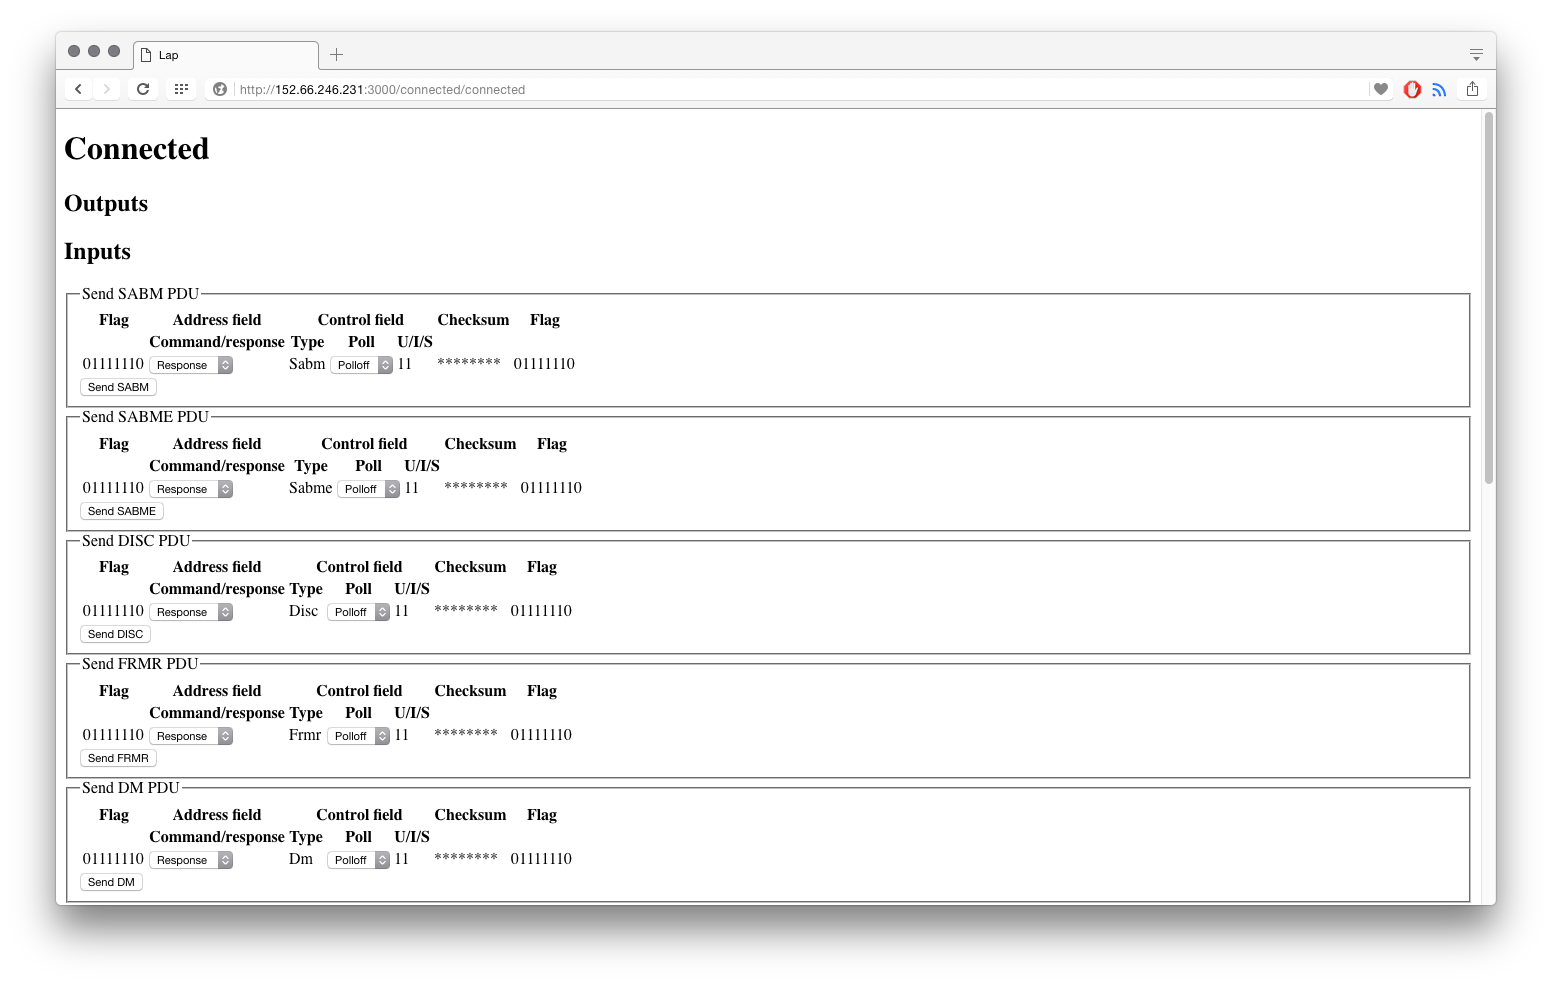
\includegraphics[width=\textwidth]{figures/web.png}
    \caption{LAB-P over HTTP web UI}
    \label{fig:web}
\end{figure}

Debug mode can be enabled by appending \verb!/on! or \verb!/off! path component to the
URI as illustrated by Figure~\ref{fig:web2}. In debug mode the current state if the protocol entity is observable
including the sequence number values, state variables, timer states, message queue contents etc.

\begin{figure}[!htb]
    \centering
    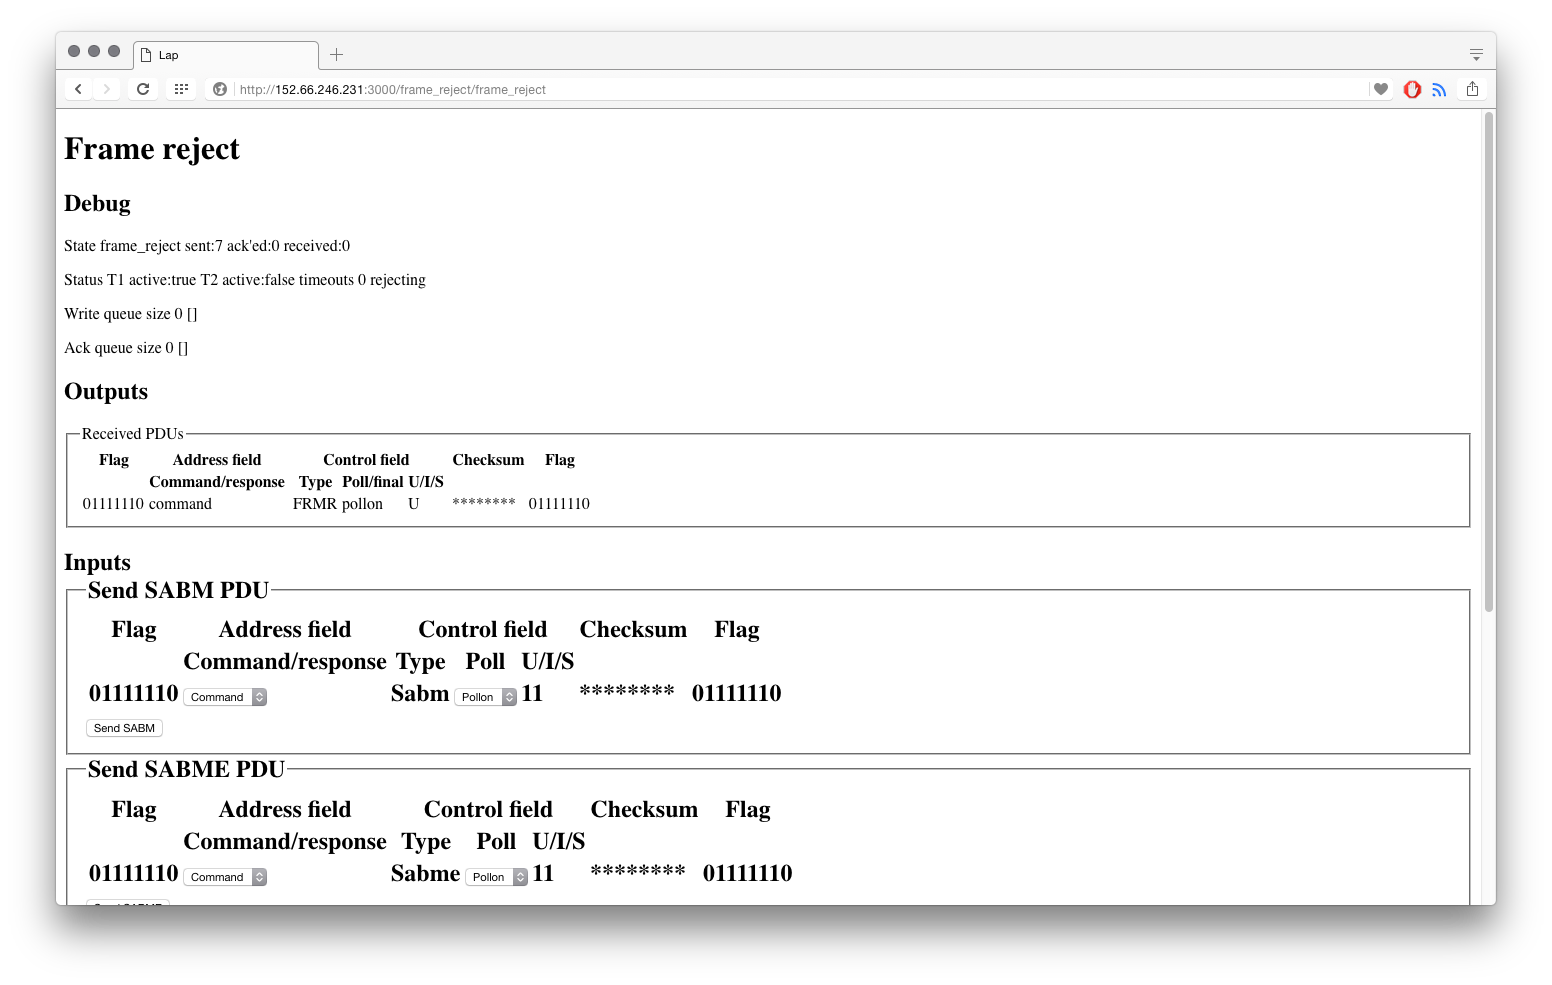
\includegraphics[width=\textwidth]{figures/web2.png}
    \caption{LAB-P over HTTP web UI in debug mode}
    \label{fig:web2}
\end{figure}

\subsection{JSON API}
In order to ease the automation of testing the web portal its JSON API is going to be used for interacting with it.

\subsection{JSON requests}\label{sec:json_req}

The JSON requests has to be addressed to the web server in embedded in a HTTP POST message body with
\verb!application/json! MIME type specified as Content-Type parameter. For example the following console command
can be used for doing so:

\begin{verbatim}
curl -H "Content-Type: application/json" \
-X POST \
-d '{"session": "a", "frame": 
{ "cr": "command", "pf": "polloff",  "type": "sabm"}}' \
http://152.66.246.231:3000/disconnected/sabm.json
\end{verbatim}

The format of the HTTP request URI path portion is the form of \url{<state>/<message type>}. For example
\url{http://152.66.246.231:3000/disconnected/sabm}. The possible state - message type combinations are listed in the
following table:

{\scriptsize
\begin{center}
    \begin{tabular}[h]{|l|l|l|}
        \hline
        Path                        & State         & Message             \\
        \hline
        \verb'connected/sabm' & connected     & SABM                \\
        \hline
        \verb'connected/sabme' & connected     & SABME               \\
        \hline
        \verb'connected/disc' & connected     & DISC                \\
        \hline
        \verb'connected/dm' & connected     & DM                  \\
        \hline
        \verb'connected/rnr' & connected     & RNR                 \\
        \hline
        \verb'connected/rr' & connected     & RR                  \\
        \hline
        \verb'connected/rej' & connected     & REJ                 \\
        \hline
        \verb'connected/i' & connected     & I                   \\
        \hline
        \verb'connected/frmr' & connected     & FRMR                \\
        \hline
        \verb'connected/t1' & connected     & T1 timeout          \\
        \hline
        \verb'connected/t2' & connected     & T2 timeout          \\
        \hline
        \verb'connected/connect_request' & connected     & connect request     \\
        \hline
        \verb'connected/disconnect_request' & connected     & disconnect request  \\
        \hline
        \verb'connected/data_request' & connected     & data request        \\
        \hline
        \verb'connecting/sabm' & connecting    & SABM                \\
        \hline
        \verb'connecting/sabme' & connecting    & SABME               \\
        \hline
        \verb'connecting/disc' & connecting    & DISC                \\
        \hline
        \verb'connecting/ua' & connecting    & UA                  \\
        \hline
        \verb'connecting/dm' & connecting    & DM                  \\
        \hline
        \verb'connecting/t1' & connecting    & T1 timeout          \\
        \hline
        \verb'connecting/connect_request' & connecting    & connect request     \\
        \hline
        \verb'connecting/disconnect_request' & connecting    & disconnect request  \\
        \hline
        \verb'connecting/data_request' & connecting    & data request        \\
        \hline
        \verb'disconnected/sabm' & disconnected  & SABM                \\
        \hline
        \verb'disconnected/sabme' & disconnected  & SABME               \\
        \hline
        \verb'disconnected/disc' & disconnected  & DISC                \\
        \hline
        \verb'disconnected/t1' & disconnected  & T1 timeout          \\
        \hline
        \verb'disconnected/connect_request' & disconnected  & connect request     \\
        \hline
        \verb'disconnected/disconnect_request' & disconnected  & disconnect request  \\
        \hline
        \verb'disconnected/data_request' & disconnected  & data request        \\
        \hline
        \verb'disconnecting/sabm' & disconnecting & SABM                \\
        \hline
        \verb'disconnecting/sabme' & disconnecting & SABME               \\
        \hline
        \verb'disconnecting/disc' & disconnecting & DISC                \\
        \hline
        \verb'disconnecting/ua' & disconnecting & UA                  \\
        \hline
        \verb'disconnecting/dm' & disconnecting & DM                  \\
        \hline
        \verb'disconnecting/i' & disconnecting & I                   \\
        \hline
        \verb'disconnecting/rej' & disconnecting & REJ                 \\
        \hline
        \verb'disconnecting/rnr' & disconnecting & RNR                 \\
        \hline
        \verb'disconnecting/rr' & disconnecting & RR                  \\
        \hline
        \verb'disconnecting/t1' & disconnecting & T1 timeout          \\
        \hline
        \verb'disconnecting/connect_request' & disconnecting & connect request     \\
        \hline
        \verb'disconnecting/disconnect_request' & disconnecting & disconnect request  \\
        \hline
        \verb'disconnecting/data_request' & disconnecting & data request        \\
        \hline
        \verb'frame_reject/sabm' & frame reject  & SABM                \\
        \hline
        \verb'frame_reject/sabme' & frame reject  & SABME               \\
        \hline
        \verb'frame_reject/t1' & frame reject  & T1 timeout          \\
        \hline
        \verb'frame_reject/connect_request' & frame reject  & connect request     \\
        \hline
        \verb'frame_reject/disconnect_request' & frame reject  & disconnect request  \\
        \hline
        \verb'frame_reject/data_request' & frame reject  & data request        \\
        \hline
    \end{tabular}
\end{center}
}

\subsection{JSON requests format}

The format of the JSON requests -- in case of \verb!curl! found after \verb!-d!
switch -- is the following for an unnumbered LAP-B frame:
\begin{verbatim}
{
"session":"a", 
"frame": 
  {
  "cr": "command", 
  "pf": "polloff", 
  "type":"sabme"
  }
}
\end{verbatim}

The JSON request format for a supervisory LAP-B frame is the following:
\begin{verbatim}
{
"session":"a", 
"frame": 
  {
  "cr": "command", 
  "pf": "polloff", 
  "type":"rr",
  "nr":6
  }
}
\end{verbatim}

The JSON format of LAP-B I frame is:
\begin{verbatim}
{
"session": "a", 
"frame": 
  {
  "cr":"command",
  "pf":"pollon",
  "type":"i",
  "nr":6,
  "ns":0
  }
}
\end{verbatim}

The \verb!session! is designated for separating student HTTP sessions so that each user has its own state
machine, state variables, etc. For this reason use the Neptun ID as session value!  The \verb!frame! is
a simplified version of a LAP-B
frame in JSON format. The \verb!cr! is the Command/Response bit from the address field, the allowed
values are \verb!command! or \verb!response! depending on the actual frame type. The
\verb!pf! is the Poll/Final bit from the control field, the value varies between
\verb!pollon! and \verb!polloff! depending on the actual frame. The
\verb!type! is the type of the LAP-B frame valid values are \verb!i!,
\verb!rr!, \verb!rnr!, \verb!rej!,
\verb!sabm!, \verb!sabme!, \verb!disc!, \verb!dm!,
\verb!ua! or
\verb!frmr!. In case of supervisory or information frames there is an additional field in the JSON
object called \verb!nr! that holds an integral value.
In case of an I frame there is also a \verb!ns! entry also with an integral value.

\subsection{JSON response format}

The format of the JSON response messages is the following:
\begin{verbatim}
{
"state": "<state>",
"error": "<error message>",
"pdu":[
  {
  "address_field":"a",
  "type":"i",
  "nr": 0,
  "ns": 3,
  "pf": "pollon",
  "cr": "response"
  }
]
"sdu":
  [
    "data_indication"
  ]
}
\end{verbatim}

The name of the next state is represented by the \verb!state! entry in the response object in string
format with potential values as the name of the states namely
\verb!connected!,
\verb!connecting!, \verb!disconnected!,
\verb!disconnecting! and \verb!frame_reject!.
If there was an error then the response object will have an entry with \verb!error! key having a string
value representing the error text.
The \verb!pdu! field has a JSON array as value containing the LAP-B frames whose structure matches
the structure of the \verb!frame! field in the request JSON object.
The \verb!address_field! will match with the request \verb!session! value. It is deliberately not
present on the HTTP response level as the system can generate more than 1 response messages as a result of one request
message. If a service primitive is invoked during the communication it will be present in the
\verb!sdu! array in string format.

Here is an example of a server generated response message:
\begin{verbatim}
{
"state":"connected",
"pdu":
  [
    {
      "address_field":"a",
      "type":"ua",
      "pf":"polloff",
      "cr":"response"
    }
  ]
}
\end{verbatim}

\section{Development and test execution environment overview}

\subsection{Development environment overview}

The dev and test execution environment is a TITAN Eclipse plugin that can be started by clicking on the Eclipse icon on the VM's desktop.

\begin{figure}[H]
  \centering
  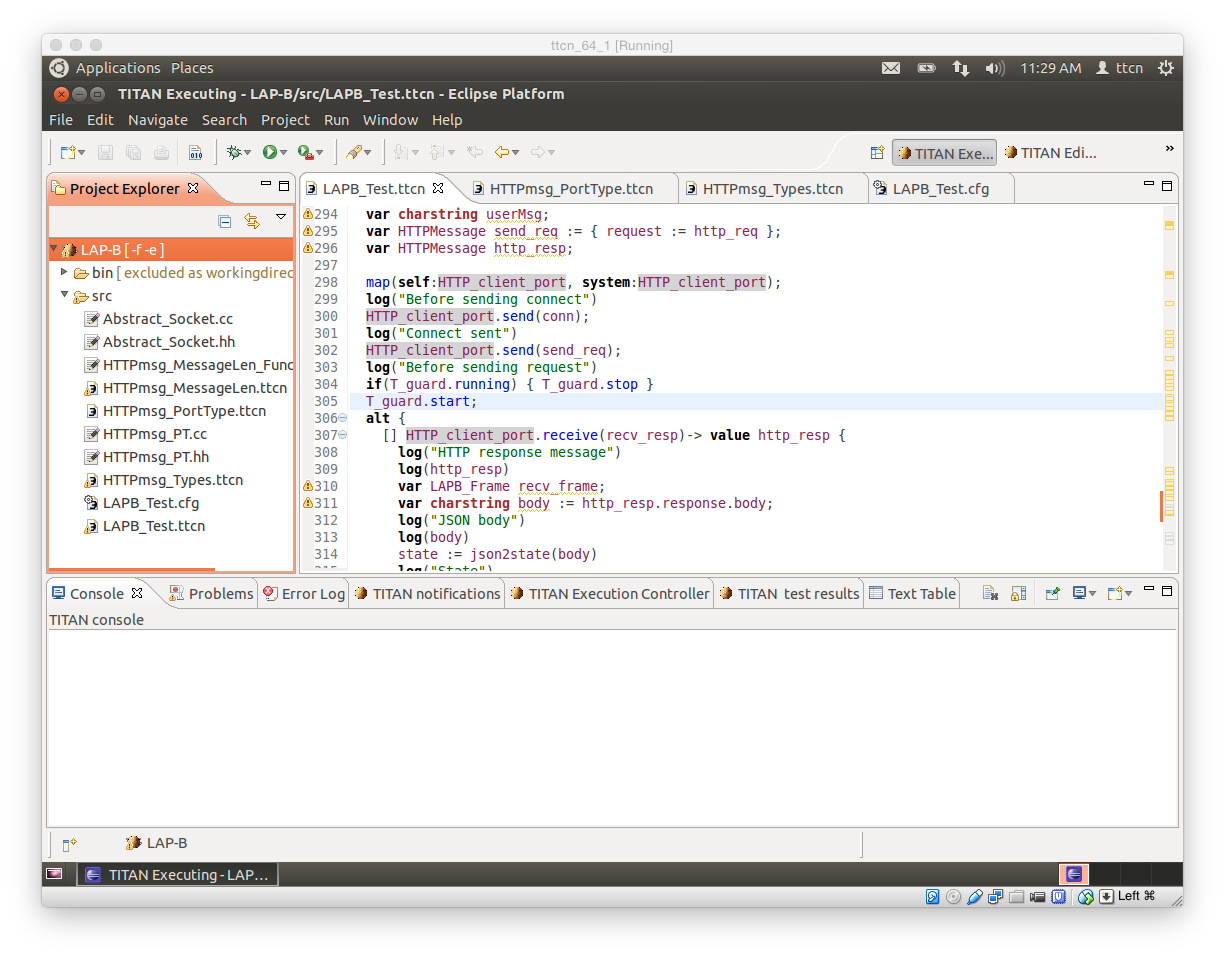
\includegraphics[width=\textwidth]{figures/eclipse.png}
  \caption{Development and test execution environment UI}
  \label{fig:eclipse}
\end{figure}

After launching the application a project will be auto opened that contains test cases whose sources have to be modified during this lab. The UI is shown on Figure~\ref{fig:eclipse}.

There are two perspectives available on the right side of the toolbar:
\textit{TITAN Executing perspective} and \textit{TITAN Editing perspective} labels, the former is used during this lab. The \textit{Project explorer} pane on the left shows the project sources, the binaries compiled from them and also the log files. The central pane contains the sources to be modified, only \verb!LAPB_Test.ttcn! file is the candidate for modification, the other files contain API and configuration settings.
The logs on message exchanges will be visible in the bottom part of the UI. 

\subsection{Building, running, logging}

The executable binary can be built from the TTCN-3 sources -- after selecting the build candidate project in the \textit{Project Explorer} view -- either from the \textit{Project} menu or from the context menu available when right-clicking on the project's name and selecting \textit{Build Project} (see Figure~\ref{fig:build}).

\begin{figure}[H]
  \centering
  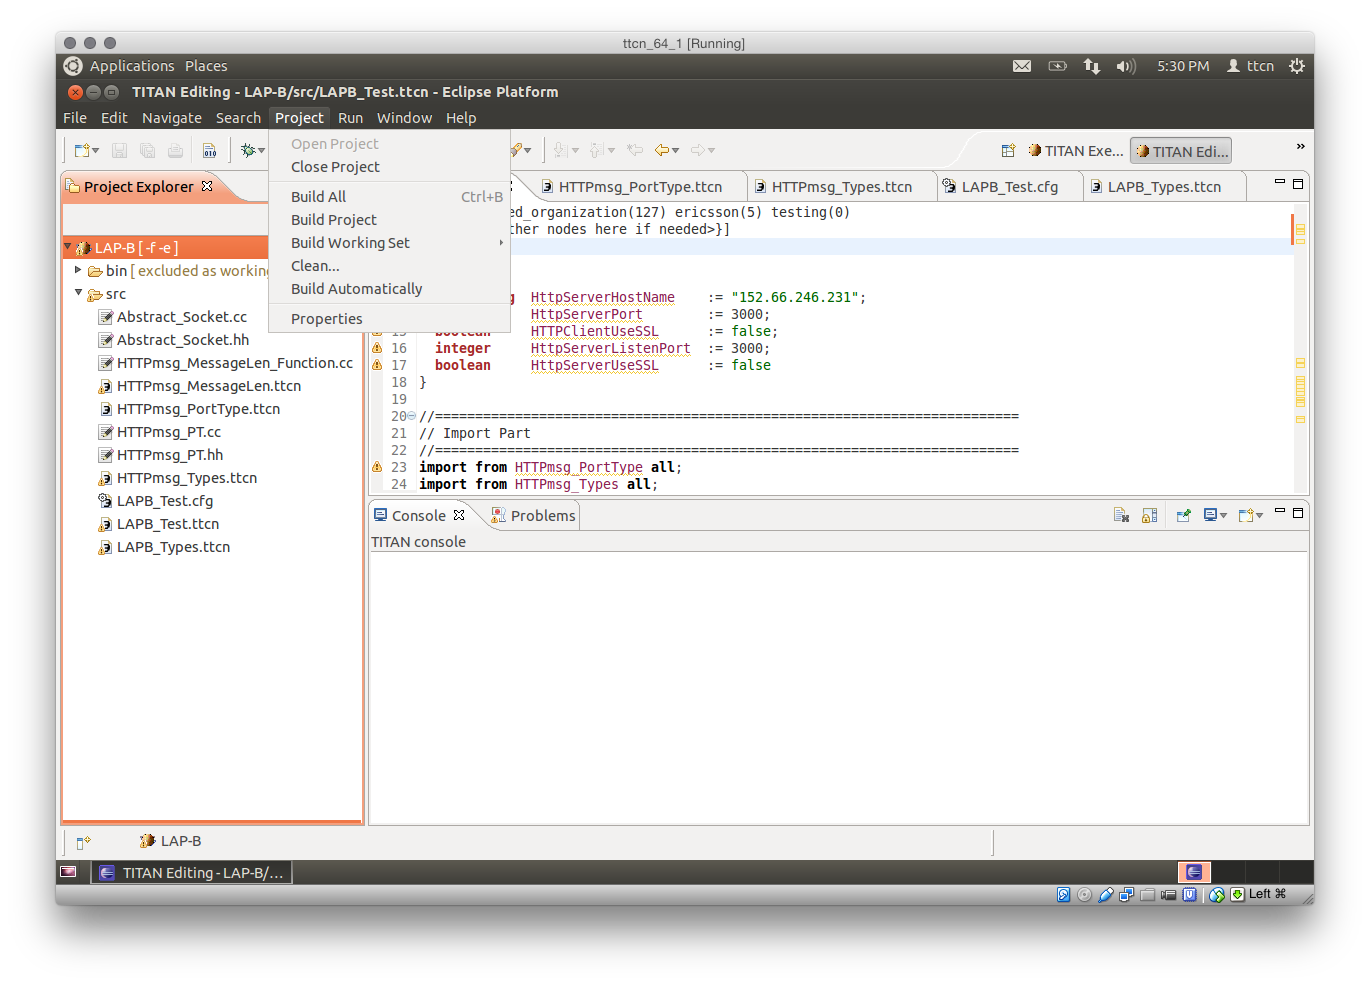
\includegraphics[width=\textwidth]{figures/build.png}
  \caption{Building the project, take caution that the right project has been selected}
  \label{fig:build}
\end{figure}

To run the executable right-click on the file \textit{LAPB{\textunderscore}Test.cfg} in the project sources in \textit{TITAN Executing perspective} view and select \textit{Run as}/\textit{TITAN Parallel launcher} from the pop-up menu.(Figure~\ref{fig:run}.)
The run results will be available on the \textit{TITAN Notifications} tab in the bottom. The log file will be available in the \textit{log} directory amongst the \textit{Project explorer} binaries. Those can be opened by double clicking on them.

\begin{figure}[H]
  \centering
  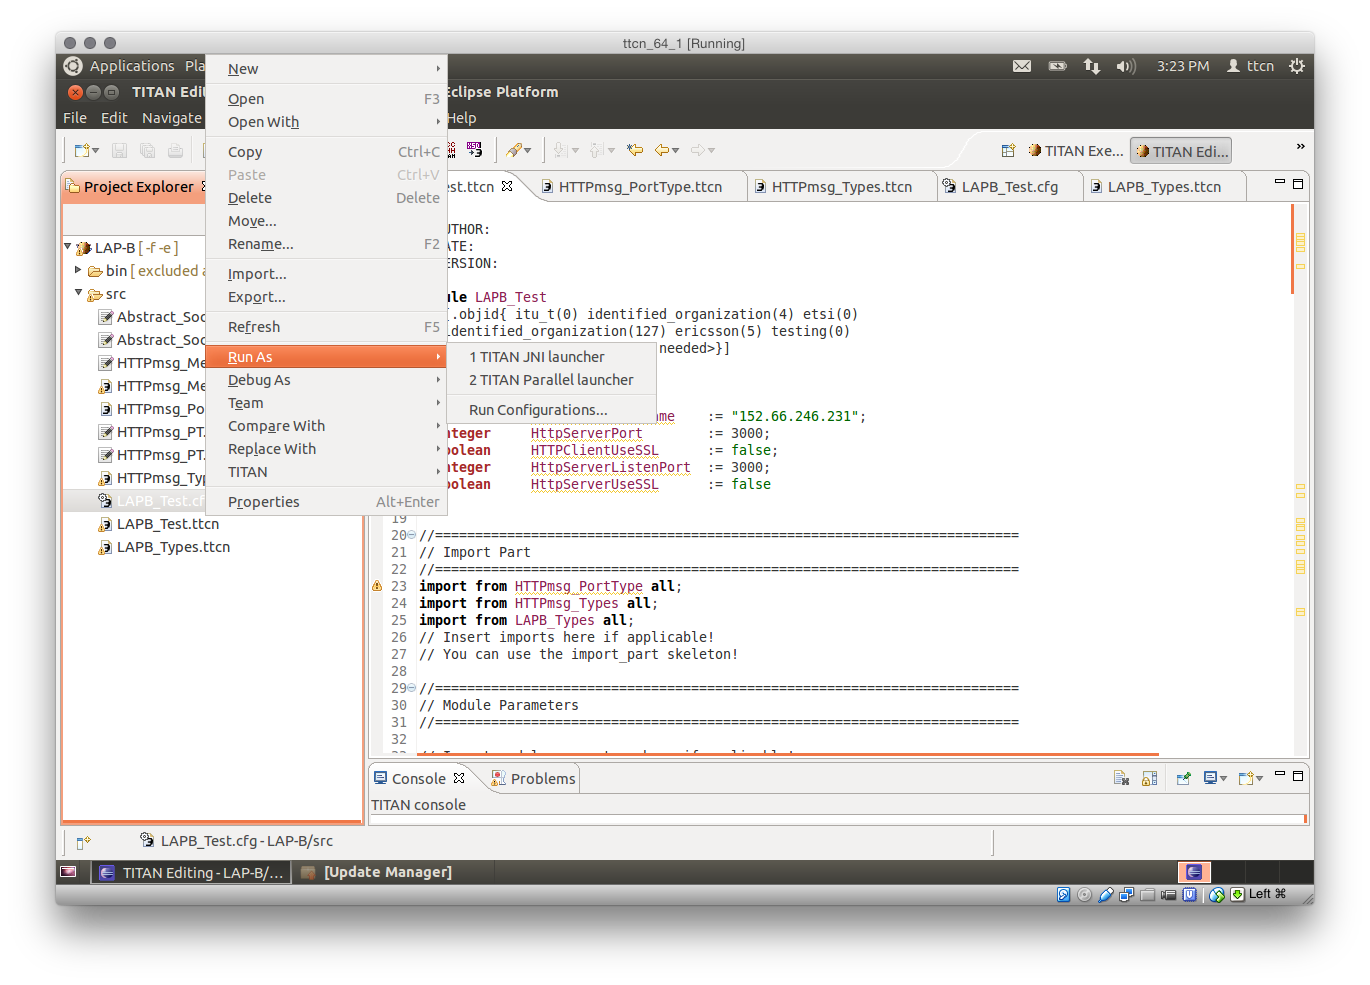
\includegraphics[width=\textwidth]{figures/run.png}
  \caption{Running the project}
  \label{fig:run}
\end{figure}

The log is in tabular format as illustrated by Figure~\ref{fig:log}. It is advised to turn on filtering by clicking on the funnel icon and filter for user events. In that case only the results of \verb!log()! calls from the source code will be visible with the corresponding JSON document.

\begin{figure}[H]
  \centering
  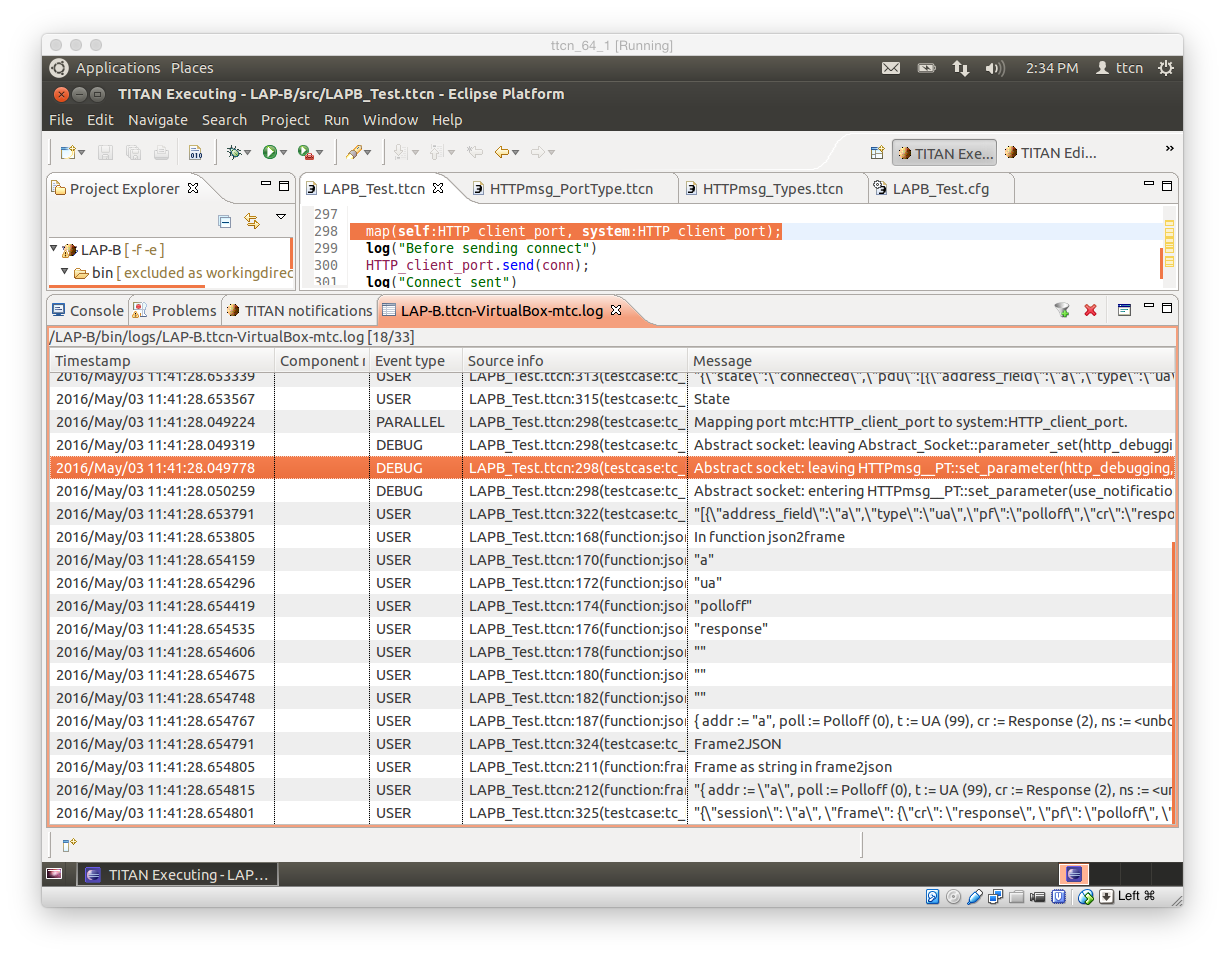
\includegraphics[width=\textwidth]{figures/log.png}
  \caption{Examining the log file of a test execution}
  \label{fig:log}
\end{figure}

\section{TTCN-3 basics}
\subsection{TTCN-3}
TTCN-3 programming language is specifically designed for describing conformance tests. Its syntax resembles C++, there are many similarities between them however it contains some language constructs that can be used to express higher level concepts that can be used for efficient description of conformance testing specific behavior. TTCN-3 is an abbreviates Testing and Test Control Notation version 3. The full specification can be found in the ETSI TTCN-3 standard \cite{ttcn3}
\footnote{\url{http://www.ttcn-3.org/index.php/downloads/standards}}.

The top level construct of a TTCN-3 code is called module. Source code is composed from modules. A module has two main parts: the definition and the control parts. In the definition part are the type declaration of the messages exchanged with SUT, the definitions of concrete messages to be send, the definition of templates used for verifying received messages furthermore the declarations of the test ports and test components used. Also here can be found the definitions of the test cases and functions describing the dynamic behavior of the tests. The control part of the module contains the test case calls necessary for executing the test.

\subsubsection{Variable and constants}

Variables can be declared in the following way in TTCN-3:

{\footnotesize
\begin{lstlisting}
var integer myVariable;
\end{lstlisting}
}

The initial value can be specified at declaration or later:
{\footnotesize
\begin{lstlisting}
myVariable := 1;
\end{lstlisting}
}

Constant values have to be initialized after declaration their value remain unchanged during test execution:

{\footnotesize
\begin{lstlisting}
const integer myConstant := 1;
\end{lstlisting}
} 

Variables can be declared in control part, test cases and inside functions and also in test component types declarations. Variable declaration in the definition part is not allowed, TTCN-3 doesn't support global variables. Constants can be defined both in definition and control sections.

\subsubsection{Importing definition from other modules}
TTCN-3 supports importing other module's definitions in a module definition section so that the imported definitions can be used there. For this \verb.import. keyword has to be used:
{\footnotesize
\begin{lstlisting}
import from MyModule all;
\end{lstlisting}
}

\subsubsection{Data types and type conversion}
TTCN-3 supports primitive and composite types.
The most important primitive types are:
{\footnotesize
\begin{center}
\begin{tabular}{|l|}
\hline
\verb/integer/ \\
\hline 
\verb/float/ \\
\hline
\verb/boolean/ \\
\hline 
\verb/bitstring/ \\
\hline 
\verb/charstring/ \\
\hline 
\verb/verdicttype/ \\
\hline
\verb!enumerated! \\
\hline
\end{tabular}
\end{center}
}

Most of these types can be found in other programming languages however \verb!verdicttype! is a TTCN-3 specific type that holds the value of the conformance test result of the SUT.

TTCN-3 composite types are:

{\footnotesize
\begin{center}
\begin{tabular}{|l|l|} 
\hline
\verb!record! & field order is fixed\\
\hline
\verb!record of! & field order fixed, homogeneous collection (e.g. \verb!record of integer!)\\
\hline
\verb!set! & fields are unordered\\
\hline
\verb!set of! & fields are unordered, homogeneous collection (e.g. \verb!set of float!)\\
\hline
\verb!union! & only one of its field can have a value\\
\hline
\end{tabular}
\end{center}
}

Example for defining composite types:
{\footnotesize
\begin{lstlisting}
type record MyRecordType{
  charstring city,
  integer district optional
}
type set MySetType{
  charstring city,
  integer district optional
}
type union MyUnionType{
  charstring passport-no,
  charstring personal-ID
}
type enumerated MyEnumeratedType{male, female}
\end{lstlisting}
}

The \verb!optional! keyword indicates that the it is not mandatory to have a value for that field.

The next example illustrates how to declare a \verb!record of! type and how to set a value of it (\verb!set of! works similarly):
{\footnotesize
\begin{lstlisting}
type record of integer MyIntegerListType;
var MyIntegerListType myIntegerList := {1, 4, 6, 5, 2}
\end{lstlisting}
}

Data types can be declared in the definition section.

During this lab these type conversion functions will be used in TTCN-3:

{\footnotesize
\begin{tabular}{|l|l|}
\hline
Integer to char string &\verb.int2str.\\
\hline
Char string to Integer  &\verb.str2int.\\
\hline
\end{tabular}
}

{\footnotesize
\begin{lstlisting}
int2str(65) == "65"
str2int("65") == 65
\end{lstlisting}
}

\subsubsection{Operators and control structures}
Just like in other languages in TTCN-3 we build expressions out of variables, literals and values. The most frequently used operators in expressions are:

{\footnotesize
\begin{tabular}{{|l|l|l|l|}}
\hline
  + &addition& != &not equal\\
\hline
 \& & string concatenation &>& greater\\
\hline
- &subtraction &<& less\\
\hline
* &multiplication &>= &greater or equal\\
\hline
/ &division &<=& less or equal\\
\hline 
== &equal &:= &assignment\\
\hline
\end{tabular}
}


The syntax of TTCN-3 control structures:


{\footnotesize
\begin{tabular}{{|l|l|l|l|}}
\hline
\verb/if/-\verb/then/-\verb/else/-structure & \verb/if (condition) {...} else {...}/\\
\hline
\verb.for.-loop & \verb/for (start;end;increment) {...}/\\
\hline
\verb/while/-loop & \verb/while (condition) {...}/\\
\hline
\verb/do/-\verb/while/-loop &\verb/do {...} while (condition)/\\
\hline
\end{tabular}
}



\subsubsection{Templates}
Templates has dual purpose. We can use them to define a sent message that matches an already defined type or to describe patterns that can be used for verifying messages arriving from the SUT.
Here's an example for defining a template based on the above declared \verb/MyRecordType/
{\footnotesize
\begin{lstlisting}
template MyRecordType myTemplate := {
  city := "Budapest",
  district := 2
}
\end{lstlisting}
}

\verb/MyRecordType/ has record type as a consequence it is not necessary to specify the name of the fields when defining a template, it's also adequate to provide values in order:
{\footnotesize
\begin{lstlisting}
template MyRecordType myTemplate := {"Budapest", 2}
\end{lstlisting}
}

For set types qualified assignment has to be used:
{\footnotesize
\begin{lstlisting}
template MySetType mySet := {
  city := "Budapest",
  district := 2
}
\end{lstlisting}
}

Example for pattern matching for messages arriving from the SUT
{\footnotesize
\begin{lstlisting}
template MyRecordType myPattern1 := {
  city := "Budapest",
  district := ?
}
\end{lstlisting}
}

It is possible to validate incoming messages against this template.
In the template definition the \verb/?/ character means that the field can have any value but it must be present in the incoming message.

If we'd like to allow that the district field can be omitted from the message we can replace \verb/?/ with \verb/*/ :
{\footnotesize
\begin{lstlisting}
template MyRecordType myPattern2 := {
  city := "Budapest",
  district := *
}
\end{lstlisting}
}

For omitting optional values \verb/omit/ keyword can be used:
{\footnotesize
\begin{lstlisting}
template MyRecordType myIncomingMessage3 := {
  city := "Budapest",
  district := omit
}
\end{lstlisting}
}

A subclass of templates are parametrized templates whose parameters can be specified during runtime:

{\footnotesize
\begin{lstlisting}
template MyRecordType myParTemplate (integer myParameter) := {
  city := "Budapest",
  district := myParameter
}
\end{lstlisting}
}

A template like this can be useful for sending 23 different templates successively without having to define 23 different templates. The value of district can be set based on the value of a loop iterator.

\subsubsection{Communication ports}

The test components can communicate with each other and the SUT using ports. A port's responsibility is to send and receive messages. To send a message execute \verb/portName.send/ \verb/(value)/ and to receive call execute \verb/portName.receive/ \verb/(templateName)/. Send operation is considered completed right after execution \verb/send/ while verb/receive/ operation a blocking operation.

A port type can be define in the following way:
{\footnotesize
\begin{lstlisting}
type port MyPort message {
  in integer, boolean;
  out bitstring;
  inout charstring
}
\end{lstlisting}
}

This declares a port that communicates with \verb/message/s that can receive integer or boolean values, can send bit strings and can both send and receive charstrings.

\subsubsection{Test components}
A test component implements a specific behavior towards the SUT. For example when testing a HTTP server test components can emulate individual user software components connecting to the server.
Components can communicate with each other and the SUT through their ports. The collection of test components create the test configuration. Based on their role we distinguish two types of test components: MTC -- Main Test Component -- and PTC -- Parallel Test Component. There can only be one MTC in a test environment. During this lab we won't use PTC as a consequence thew won't be detailed any further.

\begin{figure}[H]
  \centering
  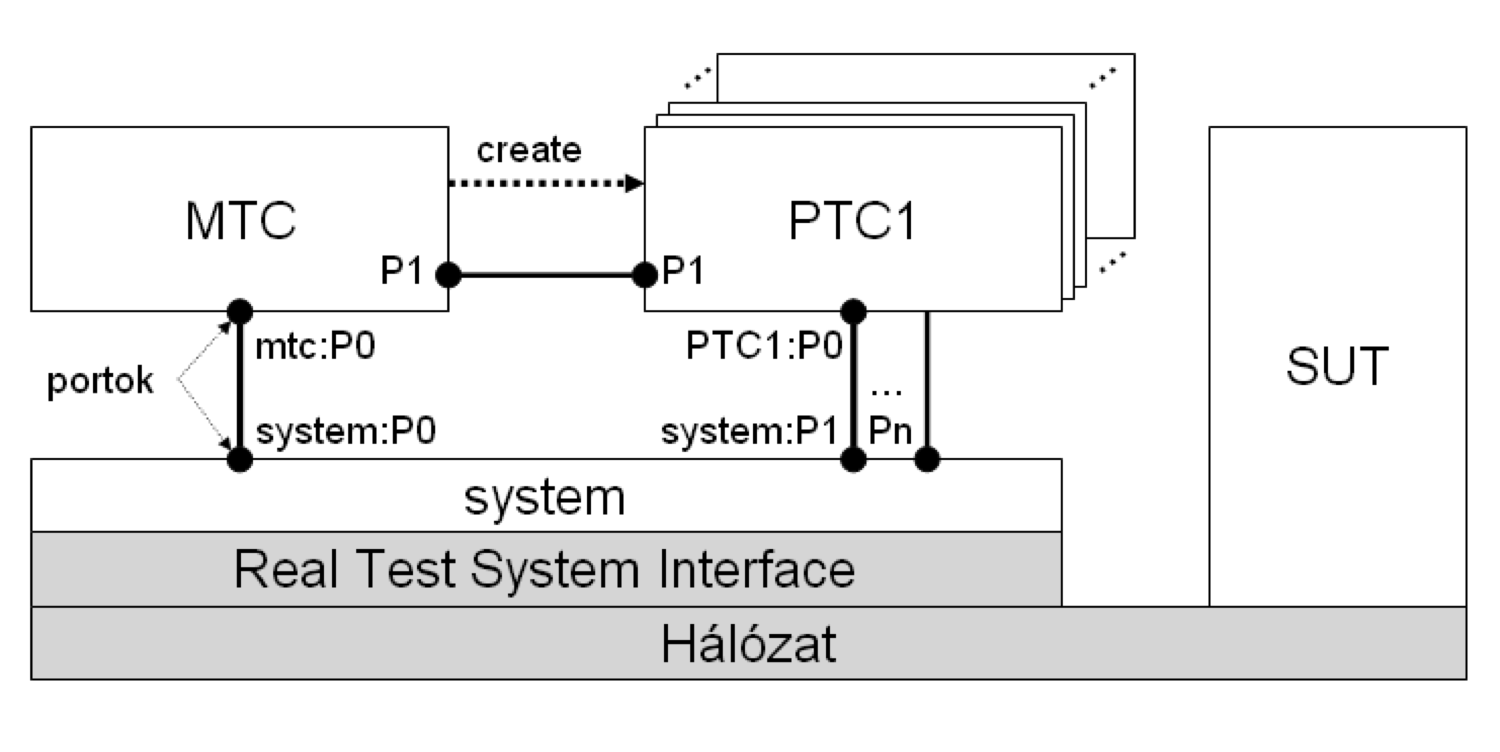
\includegraphics[width=\textwidth]{figures/TC.png}
  \caption{Test configuration}
  \label{fig:tc}
\end{figure}

The following example illustrates how to create a component containing 2 ports:

{\footnotesize
\begin{lstlisting}
type component MyComponentType{
  port MyPort P0;
  port MyPort P1;
  timer MyTimer T1;
  var MyVar v1
}
\end{lstlisting}
}

\subsubsection{Building the test configuration}

The test environment dynamic behavior can be described using functions, test cases, timers and alternative behavior branching. Before the test environment can send and receive messages the test case running on MTC has to have a valid test configuration. In this case that means to interconnect the corresponding \verb!mtc! and \verb!system! ports using the \verb/map/ statement : e.g. \verb!map(mtc: p1, system: p1)!.

The components can be referenced using the following references:

{\footnotesize
\begin{tabular}{|l|p{11cm}|}
\hline
 \verb/mtc/ &Reference to MTC\\
\hline
 \verb/self/ &Reference from the component to itself\\
\hline
 \verb/system/ &Reference to the SUT\\
\hline
\end{tabular}
}


The \verb/system/ is responsible for mapping the Real Test System Interface (RTS) and abstract world described in TTCN-3.
The RTS can be connected directly through the network to the SUT.
All this ends up in being able to only observe test configuration until the \verb/system/ boundary. During this lab we have to only deal with this abstract component.

\subsubsection{Idõzítõk}
Timers can be declared using the \verb/timer/ keyword and their value is specified in seconds using a \verb.float. Example:
{\footnotesize
\begin{lstlisting}
timer T0 := 2.0;
T0.start;
timer T1;
T1.start(2.0)
\end{lstlisting}
}

The timer can be stopped using the \verb/timerName.stop/.
To block on a timer one can use the \verb!timerName.timeout! function.

\subsubsection{Alternative behavior}

A TTCN-3 nyelv egyik legfontosabb, a tesztkomponensek, a SUT válaszától függõ, alternatív
viselkedésének leírását lehetõvé tévõ vezérlési szerkezete az \verb.alt. utasítás. Akkor használjuk,
ha a teszt végrehajtása egy olyan pontra ér, ahonnan több módon is továbbhaladhat, attól
függõen, hogy a tesztelt rendszer milyen választ küld, ha egyáltalán küld választ. Például
képzeljük el azt az egyszerû esetet, mikor a tesztelt rendszer sikeres konformancia-tesztje
azon áll, vagy bukik, hogy a legutóbb kiküldött \textit{keres} üzenetre mint gerjesztésre a
\textit{jovalasz} vagy a \textit{rosszvalasz} üzenetet küldi-e vissza. Amennyiben nem érkezik
válasz \verb/1/ másodpercen belül, a teszt kimenetele inkonkluzív lesz. A következõ kódrészlet
szemlélteti a fent leírt mûködést:

{\footnotesize
\begin{lstlisting}
timer T0;
P0.send("keres");
T0.start(1.0);
alt {
  [] P0.receive("jovalasz") {setverdict(pass);}
  [] P0.receive("rosszvalasz") {setverdict(fail);}
  [] T0.timeout {setverdict(inconc);}
}
\end{lstlisting}
}

Valamennyi \verb/alt/-ág egy szögletes zárójelekbe zárt õrfeltétellel (guard) kezdõdik, amely ha
nem teljesül, a mögötte levõ ágat egyszerûen nem vesszük figyelembe. Ha az õrfeltétel üres,
mindig teljesül. 

Az õrfeltétel után áll az
az esemény (event), amely bekövetkezte esetén az esemény után kapcsos zárójelben lévõ
utasítássorozatot végrehajtva, majd az \verb/alt/-szerkezetet elhagyva folytatódik a végrehajtás.
Amennyiben az adott ág végrehajtása után nem kívánjuk elhagyni az \verb/alt/-szerkezetet, hanem
az elejére kívánunk ugrani, úgy az adott ágon szereplõ utasítások után egy \verb/repeat/ utasítást
kell elhelyeznünk.

Ezek után vizsgáljuk meg kicsit közelebbrõl az \verb/alt/ utasítás mûködését! Nagyon fontos
megjegyezni, hogy egy \verb/alt/ utasítás nem olyan, mint az \verb/if..then..else/ szerkezet, abban
az értelemben, hogy az utasítást elérve még nem tudjuk, merre fogunk továbbhaladni. Amikor
a tesztvégrehajtás egy ilyen pontra ér, egy pillanatkép (snapshot) készül a rendszer állapotáról,
amely tartalmazza portok bemeneti sorait, valamint a változók és az idõzítõk értékeit. Ezek után kiszûrjük
azon ágakat, amelyek õrfeltétele a pillanatkép szerint igaz, azaz az aktív ágakat, amelyek közül
az elsõ olyat választjuk ki és hajtjuk végre, amelyhez tartozó esemény a pillanatkép alapján bekövetkezett.

Ha egyik esemény sem
következett be, egy újabb pillanatkép készül a rendszerrõl. A végrehajtás tehát addig
blokkolódik, amíg valamely esemény be nem következik. Ha az \verb!alt!
utasításban az összes lehetséges eseményt figyelembe vesszük, akkor
nem lesz blokkolás.


\subsubsection{Az ítéletek kezelése}
A teszt futása során az \verb!mtc! kialakít egy ítéletet a tesztelt rendszerrõl. A
korábban említettek szerint egy ítélet értéke lehet \verb/none/, \verb/pass/, \verb/inconc/, \verb/fail/ valamint
\verb/error/. Ez a sorrend szigorúsági sorrendet és egyúttal egy hierarchiát is jelent az ítéletértékek
között (a \verb/none/ a legenyhébb, míg az \verb/error/ a legszigorúbb
ítélet). 

Azaz, ha valamikor hoztunk egy \verb/pass/ ítéletet, %a tesztkomponens
                                %futása során, 
azt egy \verb/fail/ ítélettel késõbb felülírhatjuk, viszont egy már meglévõ \verb/fail/ ítéletet egy
késõbbi \verb/pass/ ítélettel nem írhatunk felül, tehát az 
ítéletek idõrendiségétõl függetlenül mindig a legszigorúbb ítélet jut érvényre.


\subsubsection{Függvények}
A függvények szerepe kettõs a TTCN-3-ban is, akárcsak a többi programozási nyelvben.
Egyrészt kiszámolhatunk velük valamit, másrészt egy viselkedést írhatunk le velük.


Egy függvény definiálásának szintaktikáját a következõ példa
szemlélteti:
{\footnotesize
\begin{lstlisting}
function MyFunction (in integer myPar) runs on MyComponentType return charstring
{
  ...
}
\end{lstlisting}
}
A fenti példát egy ponton illeti magyarázat, méghozzá a függvény paramétereinek
megadásánál. Itt az \verb/in/ kulcsszót akkor használjuk, ha a
paraméter bemenõ paraméter (C++ \verb/const/ vagy Java \verb/final/), az \verb/out/
kulcsszót akkor, ha kimenõ, míg az \verb/inout/ kulcsszót akkor, ha
kétirányú paraméter. Az \verb/in/ kulcsszó elhagyható. 
Amennyiben a függvényt egy komponens viselkedésének leírására használjuk, és a függvény a
komponensben definiált változókat, konstansokat, idõzítõket vagy portokat használja, úgy a
\verb/runs on/ kulcsszavak után meg kell adnunk annak a komponensnek a
típusát, amelyen futni fog. Végül a \verb/return/ kulcsszóval adhatjuk meg a
függvény visszatérési értékét, ha van.


A függvény futását
leállítani a \verb/stop/ utasítással lehet.
Függvényeket a definíciós részben definiálhatunk.

\subsubsection{Tesztesetek}
A tesztesetek olyan speciális függvények, amelyek az MTC-n futnak. A teszt\-e\-se\-tek\-ben nem
használhatjuk a \verb/return/ utasítást, visszatérési értékük egy ítélet a tesztelt rendszer
megfelelõségérõl. Teszteseteket a következõképpen definiálhatunk:
{\footnotesize
\begin{lstlisting}
testcase MyTestCase() runs on MyComponentType
system MySystemType
{
  ...
}
\end{lstlisting}
}
A teszteset definiálása tehát nagyban hasonlít a függvényéhez, azzal a különbséggel, hogy a
\verb.testcase. kulcsszó vezeti be, illetve megadhatjuk a tesztelt rendszer típusát is a \verb.system.
kulcsszó után.

A teszteseteket az
\verb/execute(/ \verb/tesztesetnév(/ \verb/paraméterek))/ utasítással indíthatjuk el a modulvezérlõ részben. Ekkor automatikusan létrejön a
teszt\-e\-set fejlécében megadott típusú MTC példány, majd ezen elindul a teszteset. A
tesztesetek felelõsek a tesztkonfiguráció felépítéséért is.


Teszteseteket a definíciós részben definiálhatunk.

\subsubsection{A modulvezérlõ rész}
A modulvezérlõ részt a modulon belül a \verb/control/ kulcsszó vezeti be, ezután következik
kapcsos zárójelek között a teszteseteket indító szakasz. A teszt\-e\-se\-tek indítása az \verb/execute/
kulcsszóval történik. Egy teszteset elindításakor automatikusan létrejön az MTC, amelynek
típusa a teszteset fejlécében megadott komponenstípus.


%Változók és konstansok 
%Definíciók importálása más modulokból
%Adattípusok és típuskonverzió
%Operátorok és vezérlési szerkezetek
%Adatsablonok (template-ek) 
%Kommunikációs portok 
%Tesztkomponensek 
%A tesztkonfiguráció felépítése
%Üzenetek küldése és fogadása
% Idozítok
% Alternatív viselkedések
% Az ítéletek kezelése 
% Függvények
% Tesztesetek
% A modulvezérlo rész


%TODO: 
%- read TTCN chapter
%- collect english links that covers the topic
%- translate sample exercise
%- final readthrough and wording corrections


\section{Further Reading}

\begin{itemize}
    \item \href{https://qosip.tmit.bme.hu/foswiki/pub/Meres/OpenFlowMScMeresiSegedlet/a19-lantz.pdf}{A Network in a
              Laptop: Rapid Prototyping for Software-Defined Networks}
    \item

          \href{https://qosip.tmit.bme.hu/foswiki/pub/Meres/OpenFlowMScMeresiSegedlet/mininet-hotnets2010-final.pdf}{Presentation
              of conference proceedings on Mininet}
    \item	Mininet page: \url{http://mininet.org/}
    \item	Mininet wiki: \url{https://github.com/mininet/mininet/wiki}
    \item	Mininet introduction: \url{https://github.com/mininet/mininet/wiki/  Introduction-to-Mininet}
    \item	Mininet Python API: \url{http://mininet.org/api/hierarchy.html}
\end{itemize}

\appendix

\section{Entry quiz sample questions}

%\begin{enumerate}

%  \item  Miért nemdeterminisztikus egy távköző rendszer?
%  \item  Milyen ítéletet hozunk, ha a tesztelendő rendszer nem válaszol egy kérésre?
%  \item  Milyen esetekben hozunk inconc ítéletet?
%  \item  Mi az üzenetformátum analógiája webportál esetén?
%  \item  Mi az üzenettípus analógiája webportál esetén?
%  \item  Mi a protokoll állapotátmenet analógiája webportál esetén?
%  \item  Miért van szükség az előfeltételeket beállító eseménysorozatra egy tesztesetben?
%  \item  Milyen válaszokra kell felkészülnük egy tesztesetben egy üzenet kiküldése után?
%  \item  Hogyan kerülhet holtpontra egy rendszer?
%  \item  Mi a tesztvégrehajtás eredménye, ha a teszteset bugot tartalmaz?
%  \item  Mi a kapcsolat a TTCN-3 template-ek és típusok között?
%  \item  Mi a kapcsolat a TTCN-3 template-ek és értékek között?
%  \item  Melyik lehet az alábbi, publikus interfészen deklarált C függvény tesztelését lehetővé tevő TTCN-3 porttípus definíciójának törzse?
%     int f(const char *c)
%        in integer, out charstring
%        out integer, in charstring
%        in integer, inout charstring
%        out integer, inout charstring 
%  \item Definiáljon egy TTCN-3 rekord típust, ami képes egy válasz üzenetet tárolni! (Pontos szintakszis nem elvárt) 
%\end{enumerate}

\section{Lab exercises}

\subsection{Lab environment}

\begin{thebibliography}{9}

\bibitem{ttcn3}
ETSI,
``{ETSI} {ES} 201 873-1 3 4.1 - Methods for Testing and Specification ({MTS}); The
Testing and Test Control Notation version 3; Part 1: {TTCN-3} Core Language {TTCN-3}
Edition 3.4.1 Core Language'', 
2008.09.04.
\end{thebibliography}

\end{document}